\documentclass[12pt, a4paper, oneside]{ctexart}
\usepackage{amsmath, amsthm, amssymb, bm, xcolor, tikz, framed, graphicx, hyperref, mathrsfs}
\usepackage{pgfplots}
\pgfplotsset{compat=1.18}

\title{Quantum Mechanics Homework (Week 2)}
\author{Tang Yi \\ [学号已脱敏]}
\usepackage[a4paper, left=2cm, right=2cm, top=2cm, bottom=2cm]{geometry}
\linespread{1.3} % 行距更紧凑
\definecolor{shadecolor}{RGB}{241, 241, 255}

\newcounter{problemname}
\newenvironment{problem}
  {\begin{shaded}\stepcounter{problemname}\par\noindent\textbf{题目 \theproblemname. }}
  {\end{shaded}\par}
\newenvironment{solution}
  {\par\noindent\textbf{题目 \theproblemname 的解答. }}
  {\par}
\newenvironment{note}
  {\par\noindent\textbf{题目 \theproblemname 的注记. }}
  {\par}

\begin{document}

\maketitle

\begin{problem}
    在动量表象下，

    （1）推导一维情况下的坐标算符（仿照坐标表象下动量算符的推导过程）；

    （2）写出三维情况下薛定谔方程的具体形式，设粒子处于势场$V =\mathcal{V}(x,p)$。
\end{problem}

\begin{solution}

    （1）假设动量表象的波函数$\phi(p)$，坐标表象的波函数$\psi(x)$。由坐标变换，不难有：

    \centerline{$\psi(x) = \dfrac{1}{\sqrt{2\pi \hbar}} \displaystyle \int_{-\infty}^{+\infty} \mathrm{d}p \, \phi(p) \mathrm{e}^{ipx/\hbar}$}

    则

    \centerline{$\langle x\rangle = \displaystyle \int_{-\infty}^{+\infty} \mathrm{d}x \, x \psi^*(x) \psi(x)$}

    代入$\psi(x)$，有

    \begin{align*}
        \langle x\rangle &= \dfrac{1}{2\pi \hbar} \displaystyle \int_{-\infty}^{+\infty} \mathrm{d}x \, x \left( \displaystyle \int_{-\infty}^{+\infty} \mathrm{d}p' \, \phi^*(p') \mathrm{e}^{-ip'x/\hbar} \right) \left( \displaystyle \int_{-\infty}^{+\infty} \mathrm{d}p \, \phi(p) \mathrm{e}^{ipx/\hbar} \right) \\
        &= \dfrac{1}{2\pi \hbar} \displaystyle \int_{-\infty}^{+\infty} \mathrm{d}p'  \displaystyle \int_{-\infty}^{+\infty} \mathrm{d}p   \displaystyle \int_{-\infty}^{+\infty} \mathrm{d}x \,  \phi^*(p') x  \mathrm{e}^{-i(p'-p)x/\hbar} \phi(p)\\
    \end{align*}

    注意到
    
    \centerline{$\partial_{p'} \mathrm{e}^{-i(p'-p)x/\hbar} = -\dfrac{ix}{\hbar}\mathrm{e}^{-i(p'-p)x/\hbar}$}

    代入上式，得

    \begin{align*}
        \langle x\rangle &= \dfrac{1}{2\pi \hbar} \displaystyle \int_{-\infty}^{+\infty} \mathrm{d}p'  \displaystyle \int_{-\infty}^{+\infty} \mathrm{d}p   \displaystyle \int_{-\infty}^{+\infty} \mathrm{d}x \,  \phi^*(p') (i\hbar \partial_{p'})  \mathrm{e}^{i(p'-p)x/\hbar} \phi(p)\\
        &= \displaystyle \int_{-\infty}^{+\infty} \mathrm{d}p'  \displaystyle \int_{-\infty}^{+\infty} \mathrm{d}p   \,  \phi^*(p') (i\hbar \partial_{p'}) \delta(p'-p) \phi(p)\\
        &= \displaystyle \int_{-\infty}^{+\infty} \mathrm{d}p'  \,  \phi^*(p') (i\hbar \partial_{p'}) \phi(p') \\
        &= \displaystyle \int_{-\infty}^{+\infty} \mathrm{d}p \,  \phi^*(p) (i\hbar \partial_{p}) \phi(p)
    \end{align*}

    因此，即有$\hat{x} = i\hbar \partial_p$。

    不难验证，在动量表象下，也满足正则对易关系$[\hat{x},\hat{p}] = i\hbar$。

    （2）由薛定谔方程$i\hbar \partial_t \psi = \hat{H} \psi$类比不难写出动量表象的动力学方程：

    \centerline{$i\hbar \partial_t \phi(p) = \hat{H}(i\hbar \partial_p,p) \phi(p)$}

    代入，即：

    \centerline{$i\hbar \partial_t \phi(\vec{p},t) = \left(\dfrac{p^2}{2m} + \mathcal{V}(i\hbar \vec{\nabla}_p,p)\right) \phi(\vec{p},t)$}

    其中，$\vec{\nabla}_p := \left(\dfrac{\partial}{\partial p_x},\dfrac{\partial}{\partial p_y},\dfrac{\partial}{\partial p_z}\right)$。
\end{solution}

\begin{problem}
    设三维空间中质量为$m$的粒子在势场$V(\vec{r})$中运动，

    （1）证明粒子的能量期望值为$\langle H \rangle = \displaystyle\int w \mathrm{d}^3r$，其中能量密度

    \centerline{$w = \dfrac{\hbar^2}{2m} \vec{\nabla} \psi^* \cdot \vec{\nabla} \psi + \psi^* V(\vec{r})  \psi$}

    （2）证明能量守恒公式：

    \centerline{$\dfrac{\partial w(\vec{r},t)}{\partial t} + \vec{\nabla} \cdot \vec{s}(\vec{r},t) = 0$}
 
    其中能流密度

    \centerline{$\vec{s}(\vec{r},t) = -\dfrac{\hbar^2}{2m} \left( \dfrac{\partial \psi^*}{\partial t} \vec{\nabla} \psi +  \dfrac{\partial \psi}{\partial t} \vec{\nabla} \psi^* \right)$}
\end{problem}

\begin{solution}
    （1）
    \begin{align*}
        \langle H \rangle &= \langle \psi | \hat{H} |\psi\rangle\\
        &= \displaystyle \int \mathrm{d}^3r \, \psi^* \left( -\dfrac{\hbar^2}{2m}\nabla^2 + V(\vec{r})\right) \psi \\
        &= \displaystyle \int \mathrm{d}^3r \, \left[-\dfrac{\hbar^2}{2m}\left( \vec{\nabla} \cdot (\psi^* \vec{\nabla} \psi) - \vec{\nabla} \psi^* \cdot \vec{\nabla}\psi\right) + \psi^* V(\vec{r}) \psi \right]\\
        &= \displaystyle \int \mathrm{d}^3r \, \left[\dfrac{\hbar^2}{2m} \vec{\nabla} \psi^* \cdot \vec{\nabla}\psi + \psi^* V(\vec{r}) \psi\right] - \dfrac{\hbar^2}{2m} \displaystyle \int_{\partial \mathbb{R}^3} \mathrm{d}^2\vec{r} \,   \cdot (\psi^* \vec{\nabla} \psi)\\
        &= \displaystyle \int \mathrm{d}^3r \, \left[\dfrac{\hbar^2}{2m} \vec{\nabla} \psi^* \cdot \vec{\nabla}\psi + \psi^* V(\vec{r}) \psi\right]
    \end{align*}

    因此，证明得到能量密度为：

    \centerline{$w = \dfrac{\hbar^2}{2m} \vec{\nabla} \psi^* \cdot \vec{\nabla} \psi + \psi^* V(\vec{r})  \psi$}

    （2）在推导这一题时，将会用到：

    \centerline{$\dfrac{\partial \psi}{\partial t} = \dfrac{\hat{H}}{i\hbar} \psi$， $\dfrac{\partial \psi^*}{\partial t} = -\dfrac{\hat{H}}{i\hbar} \psi^*$}

    \centerline{$\vec{\nabla}^2 \psi = -\dfrac{2m}{\hbar^2}(\hat{H}- V) \psi$，$\vec{\nabla}^2 \psi^* = -\dfrac{2m}{\hbar^2}(\hat{H}- V) \psi^*$}

    同时，$V$作为算符$\hat{V}$时对任意$\psi$本征的，本征值记为$V$。同时由于算符是厄米的，本征值应该是实的。

    下面，我们讲对$\dfrac{\partial w}{\partial t}$变形，最终得到能流密度$\vec{s}$。
    \begin{align*}
        \dfrac{\partial w}{\partial t} &= \dfrac{\hbar^2}{2m} \left[ \vec{\nabla} \left( \dfrac{\partial \psi^*}{\partial t}\right) \cdot \vec{\nabla} \psi +\vec{\nabla} \psi^* \cdot \left( \dfrac{\partial \psi}{\partial t}\right)\right] + \dfrac{\partial \psi^*}{\partial t} V \psi + \psi^* V \dfrac{\partial \psi}{\partial t}\\
        &= \dfrac{\hbar^2}{2m} \left[ \vec{\nabla} \left( \dfrac{\hat{H} \psi^*}{-i\hbar}\right) \cdot \vec{\nabla} \psi +\vec{\nabla} \psi^* \cdot \left( \dfrac{\hat{H} \psi}{i\hbar}\right)\right] + \dfrac{\hat{H} \psi^*}{-i\hbar} V \psi + \psi^* V \dfrac{\hat{H} \psi}{i\hbar}\\
        &= -\dfrac{i\hbar}{2m}\left[ \vec{\nabla} \cdot \left(\hat{H}\psi^* \vec{\nabla}\psi - \hat{H}\psi \vec{\nabla}\psi^* \right) - \left(\hat{H}\psi^* \vec{\nabla}^2\psi - \hat{H}\psi \vec{\nabla}^2\psi^*\right)\right] + \dfrac{1}{i\hbar} \left( \psi^* V \hat{H} \psi - \hat{H}\psi^* V \psi\right) \\
        &= -\dfrac{i\hbar}{2m}\left[ \vec{\nabla} \cdot \left(\hat{H}\psi^* \vec{\nabla}\psi - \hat{H}\psi \vec{\nabla}\psi^* \right) + \dfrac{2m}{\hbar^2} \left(\hat{H}\psi^* (\hat{H}-V) \psi - \hat{H}\psi (\hat{H}-V)\psi^*\right)\right] \\
        &\,\,\,\,\,\,\,+ \dfrac{V}{i\hbar} \left( \psi^*  \hat{H} \psi - \psi \hat{H}\psi^*  \right) \\
        &= -\dfrac{i\hbar}{2m}\left[ \vec{\nabla} \cdot \left(\hat{H}\psi^* \vec{\nabla}\psi - \hat{H}\psi \vec{\nabla}\psi^* \right) + \dfrac{2mV}{\hbar^2} \left(-\psi\hat{H}\psi^*  + \psi^*\hat{H}\psi \right)\right]+ \dfrac{V}{i\hbar} \left( \psi^*  \hat{H} \psi - \psi \hat{H}\psi^*  \right)\\
        &= -\dfrac{i\hbar}{2m} \vec{\nabla} \cdot \left(-i\hbar\partial_t\psi^* \vec{\nabla}\psi - i\hbar \partial_t\psi \vec{\nabla}\psi^* \right) + \dfrac{V}{i\hbar} \left(-\psi\hat{H}\psi^*  + \psi^*\hat{H}\psi \right)+ \dfrac{V}{i\hbar} \left( \psi^*  \hat{H} \psi - \psi \hat{H}\psi^*  \right)\\
        &= \vec{\nabla} \cdot \left(\dfrac{\hbar^2}{2m} \left( \dfrac{\partial \psi^*}{\partial t} \vec{\nabla} \psi +  \dfrac{\partial \psi}{\partial t} \vec{\nabla} \psi^* \right)\right) 
    \end{align*}

    因此，证明得到能流密度为：

    \centerline{$\vec{s}(\vec{r},t) = -\dfrac{\hbar^2}{2m} \left( \dfrac{\partial \psi^*}{\partial t} \vec{\nabla} \psi +  \dfrac{\partial \psi}{\partial t} \vec{\nabla} \psi^* \right)$}
\end{solution}

\begin{problem}
    在一维情况下证明：

    \centerline{$\dfrac{\mathrm{d}\langle p\rangle}{\mathrm{d}t} = \left\langle - \dfrac{\partial V}{\partial x}\right\rangle$}
\end{problem}

\begin{solution}
    \begin{align*}
        \mathrm{LHS} &= \dfrac{\mathrm{d}}{\mathrm{d}t} \left\langle \psi \left| \hat{p} \right| \psi \right\rangle \\
        &= \left\langle \dfrac{\partial \psi}{\partial t} \left| \hat{p} \right| \psi \right\rangle + \left\langle \psi \left| \hat{p} \right| \dfrac{\partial \psi}{\partial t} \right\rangle \\
        &= \left\langle \dfrac{\psi}{i \hbar} \left| \hat{H} \hat{p} \right| \psi \right\rangle + \left\langle \psi \left| \hat{p}\hat{H} \right| \dfrac{\psi}{i \hbar} \right\rangle \\
        &= \dfrac{1}{i \hbar} \left\langle \psi \left| [\hat{p},\hat{H}] \right| \psi \right\rangle \\
        &= \dfrac{1}{i \hbar} \left( \dfrac{1}{2m}\left\langle \psi \left| [\hat{p},\hat{p}^2] \right| \psi \right\rangle + \left\langle \psi \left| [\hat{p},V(\hat{x})] \right| \psi \right\rangle \right) \\
        &= \dfrac{1}{i \hbar} \left\langle \psi \left| [\hat{p},\hat{x}] \dfrac{\partial V}{\partial x} \right| \psi \right\rangle \\
        &= \dfrac{1}{i \hbar} \left\langle \psi \left| -i \hbar\dfrac{\partial V}{\partial x} \right| \psi \right\rangle \\
        &= \left\langle \psi \left| - \dfrac{\partial V}{\partial x} \right| \psi \right\rangle = \left\langle -\dfrac{\partial V}{\partial x} \right\rangle = \mathrm{RHS}
    \end{align*}
\end{solution}

\begin{problem}
    求讲义P15中$t$时刻波函数的几率流密度，并据此分析几率密度随时间的演化。
\end{problem}

\begin{solution}
    注意到，其波函数为

    \centerline{$\Psi(x,t) = \left(\dfrac{1}{\pi}\right)^{1/4} \dfrac{1}{\sqrt{\alpha+\dfrac{i\hbar t}{m\alpha }}} \exp\left[\dfrac{ip_0}{\hbar}\left(x-\dfrac{p_0t}{m}\right)\right]\exp\left[-\dfrac{\left(x-\dfrac{p_0 t}{m}\right)^2}{2\alpha^2\left(1+\dfrac{i\hbar t}{m\alpha^2}\right)}\right]$}

    代入几率流密度：

    \begin{align*}
        j(x,t) &= \dfrac{\hbar}{2mi} \left( \Psi^* \dfrac{\partial \Psi}{\partial x} - \Psi \dfrac{\partial \Psi^*}{\partial x} \right)\\
        &= \Psi^* \Psi \left[\dfrac{p_0}{m}  + \dfrac{\hbar^2 t}{m^2 \alpha^4  \left(1 + \dfrac{\hbar^2 t^2}{m^2 \alpha^4}\right)} \left(x - \dfrac{p_0t}{m}\right)\right]\\
        &= \dfrac{1}{\sqrt{\pi \alpha^2 \left(1+\dfrac{ \hbar^2t^2}{m^2\alpha^4}\right)}} \left[\dfrac{p_0}{m}  + \dfrac{\hbar^2 t}{m^2 \alpha^4  \left(1 + \dfrac{\hbar^2 t^2}{m^2 \alpha^4}\right)} \left(x - \dfrac{p_0t}{m}\right)\right] \exp\left[  -\dfrac{\left(x - \dfrac{p_0t}{m}\right)^2}{\alpha^2 \left( 1+\dfrac{\hbar^2  t^2}{m^2\alpha^4}\right)}\right]
    \end{align*}

    分析几率流，我们将其分为两项：

    \centerline{$j(x,t) = j_1(x,t) + j_2(x,t)$}

    \centerline{$\,$}

    其中，$j_1 = \dfrac{p_0}{m} \Psi^* \Psi$，$j_2 = \Psi^* \Psi \dfrac{\hbar^2 t}{m^2 \alpha^4  \left(1 + \dfrac{\hbar^2 t^2}{m^2 \alpha^4}\right)} \left(x - \dfrac{p_0t}{m}\right)$。

    如果我们简单的认为$j = \rho v$，那么第一项$j_1$表示波包整体以速度$\dfrac{p_0}{m}$向右运动，这可以通过分析$\langle x \rangle = \dfrac{p_0 t}{m}$得到同样的结果。

    第二项$j_2$表示波包的扩散。扩散速率同时是关于高斯波包的中心对称的，$v_{\mathrm{diff}}(x,t) = \eta(t) w(x)$。其中$\eta(t) = \dfrac{\hbar^2 t}{m^2 \alpha^4  \left(1 + \dfrac{\hbar^2 t^2}{m^2 \alpha^4}\right)}$是扩散的效率，与时间有关。$w(x) = x - \dfrac{p_0t}{m}$是关于波包中心对称的线性权重，表征这样的扩散是以$x = \dfrac{p_0t}{m}$为中心，越靠边缘越快的扩散。

    \begin{center}
    \begin{tikzpicture}[scale=0.7]
    \begin{axis}[
        axis lines = left,
        xlabel = {$t$},
        ylabel = {$\eta(t)$},
        samples=200,
        domain=0:15,
        width=15cm,
        height=8cm,
        xmin=0, xmax=16,
        xtick={0,3,6,9,12,15},
        ymin=0, ymax=0.55,
        yticklabel style={/pgf/number format/fixed},
        thick,
        smooth,
        legend style={at={(0.98,0.98)},anchor=north east}
    ]
    % 设定参数
    \addplot[blue, thick] {x/(1 + x^2)};
    \addlegendentry{$\eta(t) \propto \frac{t}{1 + t^2}$};
    \end{axis}
    \end{tikzpicture}
    \end{center}


    由图可见，$\eta(t)$先增大后减小，说明扩散速率先增大后减小。结合波包的扩散，可以理解为：初始时刻波包非常集中，扩散速率较慢；随着时间推移，波包逐渐扩散，扩散速率增大；当波包已经非常分散时，扩散速率又逐渐减小。

    同时，我们还绘制了$v(t)$的图像，方便进一步展示波包的动力学演化。

    \begin{center}
        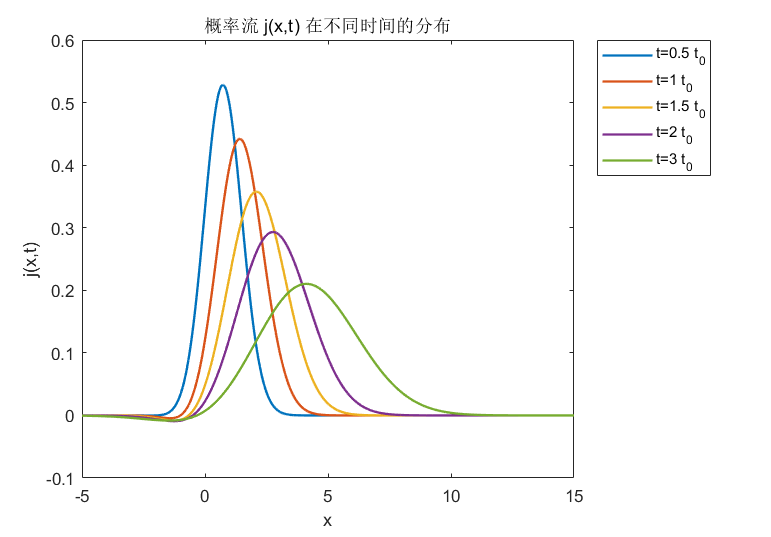
\includegraphics[width=0.85\textwidth]{pro_flux.png}
    \end{center}

\end{solution}
\begin{problem}
    假设初始时刻粒子处于状态$\Psi(x,0)=c_1\psi_1(x)+c_2\psi_2(x)$, 其中$\psi_1(x)$和$\psi_2(x)$是能量本征态, 分别属于能量本征值$E_1,E_2$， 叠加系数$c_1,c_2$已知。计算$t>0$时刻位置的期望值$\langle x\rangle(t)$ 。(设$c_1,c_2,\psi_1(x),\psi_2(x)$ 都为实数)
\end{problem}

\begin{solution}
    由题意，$t>0$时刻的波函数为：

    \centerline{$\Psi(x,t) = c_1 \psi_1(x) \mathrm{e}^{-iE_1t/\hbar} + c_2 \psi_2(x) \mathrm{e}^{-iE_2t/\hbar}$}

    则位置的期望值为：

    \begin{align*}
        \langle x\rangle(t) &= \displaystyle \int_{-\infty}^{+\infty} \mathrm{d}x \, \Psi^* x \Psi \\
        &= \displaystyle \int_{-\infty}^{+\infty} \mathrm{d}x \, x \left( c_1^2 \psi_1^2 + c_2^2 \psi_2^2 + 2c_1c_2\psi_1\psi_2\cos\dfrac{(E_2-E_1)t}{\hbar}\right)\\
        &= c_1^2 \displaystyle \int_{-\infty}^{+\infty} \mathrm{d}x \, x  \psi_1^2 + c_2^2  \displaystyle \int_{-\infty}^{+\infty} \mathrm{d}x \, x  \psi_2^2 + 2c_1c_2\cos\dfrac{(E_2-E_1)t}{\hbar}  \displaystyle \int_{-\infty}^{+\infty} \mathrm{d}x \, x  \psi_1\psi_2\\
        &= c_1^2 X_{11} + c_2^2 X_{22} + 2c_1c_2 X_{12}\cos\dfrac{(E_2-E_1)t}{\hbar}
    \end{align*}

    其中，$X_{ij} :=  \displaystyle \int_{-\infty}^{+\infty} \mathrm{d}x \, x  \psi_i\psi_j$。

    因此，$\langle x\rangle(t)$随时间做简谐振动，振幅为$2c_1c_2 X_{12}$，频率为$\dfrac{E_2-E_1}{\hbar}$。
\end{solution}
\end{document}